
%-------------------------------------------------------------------------------
\chapter{Methodology}\label{sec:methods}
\vspace{-1cm} \label{cap4}
%
%\begin{flushright}
%\begin{minipage}{0.7\linewidth}
%\emph{``Se quiser por � prova o car�ter de um homem, d�-lhe
%poder.''}
%\end{minipage}
%\end{flushright}
%
%\begin{flushright}
%{Abraham Lincoln}
%\end{flushright}
%
%\section{Introdu��o}\label{introducao_cap_3}
%\markright{\thesection ~~~ Modelos de Previs�o} \label{previsao}
%
%

This chapter narrows the field of sensor fusion under irregular sampling down to the problem of estimating the states of a system with a known process model, that is observed by aperiodically sampled measurements. We begin with a review of the adopted algorithm, that is the Kalman Filter, which is the most common approach to probabilistic data fusion. The nonlinear extension based on the unscented transform is also explored.
In Section~\ref{sec:estimation_aperiodic} we describe the particularities of the filtering algorithms for when the correct time-stamp is available to the estimator and when it is not. We end with a description of the performance criteria used for results assessment, designed to quantify estimation accuracy and consistency.


\section{Bayesian Estimation}\label{sec:bayes_estimation}

The Bayesian approach to state estimation can be interpreted as a data fusion algorithm in which the inferred knowledge about the system's states is updated continuously as new information arrives, using not just the new data, but also the prior information. For that, both the desired knowledge of the states and the continuous information are modeled as random variables (RV), hence its classification falls under the probabilistic fusion framework.

The goal of the estimator is to statistically and recursively infer the values of the system's states, the random vector $x_k \in \mathbb{R}^n$, from noisy data, the observation vector sequence $y_1,...,y_k \in \mathbb{R}^m$. The respective conditional PDF, $\rho(x_k|(y_1,...,y_k))$, is called the \textit{posterior} density function, describing the statistics of the random vector $x_k \in \mathbb{R}^n$, after the present and past experimental observations  $\rho(x_k|(y_1,...,y_k))$ have been taken. Thus we can find the estimation of $x_k \in \mathbb{R}^n$ using methods such as the \textit{maximum a posteriori} (MAP) or \textit{minimum mean square error} (MMSE), given by \citep{Bar-Shalom2001}

\begin{align}
\hat{x}_k^{MAP} &\triangleq \operatorname{arg}  \underset{x_k}{\operatorname{max}} \ \hat{\rho}(x_k|(y_1,...,y_k)), \label{eq:map} \\
\hat{x}_k^{MMSE} &\triangleq \operatorname{arg}  \underset{x_k}{\operatorname{min}} \ E[(\hat{x}_k-x_k)^T(\hat{x}_k-x_k)|(y_1,...,y_k)], \label{eq:mmse}
\end{align}

\noindent
where $\hat{x_k}$ is the estimated value of $x_k \in \mathbb{R}^n$, $\hat{\rho}(x_k|(y_1,...,y_k))$ is the estimated posterior density of $x_k$ given the observation sequence, and $E[(\hat{x}_k-x_k)^T(\hat{x}_k-x_k)|(y_1,...,y_k)]$ is the variance of the random vector $x_k$, given the observation sequence. MAP can be interpreted as the bayesian approach to \textit{maximum likelihood} (ML) estimation, whereas MMSE is the counterpart of the \textit{least squares} (LS) estimator \citep{Bar-Shalom2001}. 

Finding the \textit{posterior} $\rho(x_k|(y_1,...,y_k))$ defines the complete state estimation problem, whereas the estimates $\hat{x_k}^{MAP} \in \mathbb{R}^n$ and $\hat{x_k}^{MMSE} \in \mathbb{R}^n$ are the optimal state estimates, under their optimality criteria. A recursive Bayesian solution to the state estimation problem, that is finding the \textit{posterior} PDF, considering that the system evolves according a Markov process is presented in Proposition~\ref{prop:bayes_solution}. But first, we need to define two lemmas.

\begin{lema}\label{lemma:markov} For a Markov system with initial state $x_0 \sim \rho(x_0)$, the transition density of the future state $x_{k+1}$ given the present state $x_k$ is independent of past states, that is

\begin{equation}\label{eq:lemma_transition}
\rho(x_{k+1} | (x_0,...,x_k)) = \rho(x_{k+1}|x_k),
\end{equation}

\noindent
and observation vector $y_k$ is independent of past observations and past states, if present state $x_k$ is given, that is

\begin{equation}\label{eq:lemma_likelihood}
\rho(y_k|(x_0,...,x_k,y_0,...,y_{k-1}) = \rho(y_k|x_k).
\end{equation}
\end{lema}

\begin{lema} \label{lemma:chapman}For a Markov system, we can find the transition density from step $n$ to step $s$ as a function of the transition densities between them and an intermediate step $r$, as long as $n>r>s$, by the Chapman-Kolmogorov equation~\citep{Papoulis1984}

\begin{equation}
\rho(x_n|x_s) = \int_{-\infty}^{\infty}\rho(x_n|x_r)\rho(x_r|x_s)dx_r.
\end{equation}
\end{lema}
\vspace{0.2cm}

Note that the system described in Section~\ref{sec:problem_form} is Markovian, since the transition or process model given by (\ref{eq:prob_process}) and the observation model given by (\ref{eq:prob_obs}) follow the conditions (\ref{eq:lemma_transition}) and (\ref{eq:lemma_likelihood}), respectively.

\begin{propo}\label{prop:bayes_solution} The posterior density of system states $x_k \in \mathbb{R}^n$ conditioned on the observation vector sequence $y_1,...,y_k \in \mathbb{R}^m$ is recursively given by

\begin{align}
\rho(x_{k}|(y_1,...,y_{k-1})) &= \int_{\mathbb{R}^n}\rho(x_k|x_{k-1}) \rho(x_{k-1}|y_1,...,y_{k-1})dx_{k-1} \label{eq:prop_xk1}, 
\\ \notag \\
\rho(x_k|(y_1,...,y_k)) &= \frac{\rho(y_k|x_k) \rho(x_k | (y_1,...,y_{k-1}))}{\rho(y_k|(y_1,...,y_{k-1}))}   \label{eq:prop_xk}
\end{align}
	

\noindent
where $k \in \mathbb{N}$, $\rho(y_k|x_k)$ is the \textit{likelihood density}, $\rho(x_k|(y_1,...,y_{k-1})$ is the \textit{prior density}, defined before the latest measurement, $\rho(x_{k}|x_{k-1})$ is the \textit{transition density} that models the evolution of $x_k$ and $\rho(y_k|(y_1,...,y_{k-1}))$ is the \textit{evidence}, also referred to as normalizing factor, or marginalization. The evidence term is commonly presented as a constant~\citep{Sarkka2013}, since it does not depend on the state vector $x_k$, and it can be computed by the Chapman-Kolmogorov equation from Lemma~\ref{lemma:chapman}

\begin{align}
\rho(y_k|(y_1,...,y_{k-1}) 	&= \int_{\mathbb{R}^n} \rho(y_k|x_k)\rho(x_k|(y_1,...,y_{k-1})) dx_k, \\
							&= z_k. \notag
\end{align}
	
The algorithm is initialized by a known prior $\rho(x_0)$ and recursion is achieved by introducing the PDF calculated in the \textit{forecast} step, given by (\ref{eq:prop_xk1}), in the \textit{data assimilation} step, given by (\ref{eq:prop_xk}).
\end{propo}

\begin{proof}

The posterior PDF can be computed by the \textit{Bayes' rule}~\citep{Stone2013}

\begin{equation}\label{eq:post_pdf}
\rho(x_k|(y_1,...,y_k)) = \frac{\rho((y_1,...,y_k)|x_k)\rho(x_k)}{\rho(y_1,...,y_k)}.\\
\end{equation}

Using the definition of the conditional probability, given by ~\citep{Papoulis1984}

\begin{equation}\label{eq:cond_prob}
\rho((a_1,...,a_k)|(a_{k+1},...,a_n)) = \frac{ \rho(a_1,...,a_k,...,a_n)}{\rho(a_{k+1},...,a_n)}, \\
\end{equation}

\noindent
and the chain rule of probability, that is ~\citep{Papoulis1984}

\begin{equation}\label{eq:chain_rule}
\rho(a_1,...,a_n) = \rho(a_n|a_1,...a_{n-1})\rho(a_1,...a_{n-1}), \\
\end{equation}
\noindent
it is possible to rewrite (\ref{eq:post_pdf}) as

\begin{equation}\label{eq:post_pdf2}
\rho(x_k|(y_1,...,y_k)) = \frac{\rho(y_k|(y_1,...,y_{k-1},x_k))\rho(y_1,...,y_{k-1}|x_k)\rho(x_k)}{\rho(y_k|(y_1,...,y_{k-1}))  \rho(y_1,...,y_{k-1})}. \\
\end{equation}

From Lemma~\ref{lemma:markov}, given the current state $x_k$, the present $y_k$ is independent of past observations, thus the first term of the dividend becomes $\rho(y_k|x_k)$. Additionally, Bayes' rule in the second term yields

\begin{equation}\label{eq:post_pdf3}
\rho((y_1,...,y_{k-1})|x_k)) = \frac{\rho(x_k|(y_1,...,y_{k-1})) \rho((y_1,...,y_{k-1}))}{\rho(x_k)}.\\
\end{equation}

Finally, by combining all together, we have

\begin{equation}\label{eq:final_cond_pdf}
\rho(x_k|(y_1,...,y_k)) = \frac{\rho(y_k|x_k) \rho(x_k|(y_1,...,y_{k-1})) {\color{gray}\rho((y_1,...,y_{k-1})) \rho(x_k)}} {\rho(y_k|(y_1,...,y_{k-1}))  {\color{gray}\rho(y_1,...,y_{k-1}) \rho(x_k)}},\\
\end{equation}

\noindent
which, after canceling the equal terms (in gray), proves (\ref{eq:prop_xk}).

To prove (\ref{eq:prop_xk1}), we introduce a predicted state $x_{k+1}$ in the posterior PDF, that is $\rho(x_{k+1},x_k|(y_1,...,y_k))$ ~\citep{Bergman1999}. Rewriting the new conditional density with the aid of (\ref{eq:cond_prob}), (\ref{eq:chain_rule}) and Lemma~\ref{lemma:markov}, we have

\begin{align}
\rho(x_{k+1}, x_k | (y_1,...,y_k)) &= \rho(x_{k+1}|(x_k,y_1,...,y_k))\rho(x_k|(y_1,...,y_k)) \notag \\
&=\rho(x_{k+1}|(x_k)\rho(x_k|(y_1,...,y_k)) \label{eq:forecast_condPDF}.
\end{align}

The integration of both sides of (\ref{eq:forecast_condPDF}) with respect to $x_k$ yelds (\ref{eq:prop_xk1}), which is also a Chapman-Kolmogorov equation. This last piece of proof is also an application of Lemma~\ref{lemma:chapman}.

\end{proof}

Thus, (\ref{eq:prop_xk}) can be interpreted as the fusion of the \textit{prior} density or knowledge of the state with the \textit{likelihood} density or evidence. For a better understanding, we can illustrate this process for a one-dimensional Gaussian case \citep{Faragher2012}, for which the densities are given by
\clearpage
\begin{align}
\rho(x_k|(y_1,...,y_{k-1})) &= \mathcal{N}(x_k|\hat{x}_{prior},\hat{\sigma}_{prior}) \notag \\&= \frac{1}{\sqrt{2\pi}\hat{\sigma}_{prior}} \exp \left( - \frac{(x_k - \hat{x}_{prior})^2}{2\hat{\sigma}_{prior}^2}\right), \label{eq:prior}
\\ \notag \\
\rho(y_k|x_k) &= \mathcal{N}(y_k|x_k,\hat{\sigma}_{evidence}) \notag \\&= \frac{1}{\sqrt{2\pi} \hat{\sigma}_{evidence}} \exp \left( - \frac{(y_k - x_k)^2}{2\hat{\sigma}_{evidence}^2}\right), \label{eq:likelihood}
\end{align}

\noindent
where the \textit{prior} defined in (\ref{eq:prior}) is obtained by forecasting and the \textit{likelihood} given y (\ref{eq:likelihood}) is obtained by a linear observation model, say $y_k = x_k + w_k$, with $w_k \sim \mathcal{N}(0,\sigma_{evidence})$. Under the MAP estimation method, we can combine (\ref{eq:map}), (\ref{eq:prop_xk}) (\ref{eq:prior}) and (\ref{eq:likelihood}), discarding the normalization factor, which is independent of $x_k$, yielding

\begin{align}
\hat{x}_k^{MAP} &= \operatorname{arg}  \underset{x_k}{\operatorname{max}} \ \rho(y_k|x_k) \rho(x_k | (y_1,...,y_{k-1})) \notag  \\
&= \operatorname{arg}  \underset{x_k}{\operatorname{max}} \ \mathcal{N}(y_k|x_k,\hat{\sigma}_{evidence}) \mathcal{N}(x_k|\hat{x}_{prior},\hat{\sigma}_{prior})\notag \\
&= \operatorname{arg}  \underset{x_k}{\operatorname{max}} \ \mathcal{N}(x_k|\hat{x}_{posterior}(y_k), \hat{\sigma}_{posterior}) \\
& = \hat{x}_{posterior}(y_k),  \label{eq:posterior} 
\end{align}

\noindent where 

\begin{align}
\hat{x}_{posterior}(y_k)	 &= 
\frac{\hat{\sigma}_{evidence}^2}{\hat{\sigma}_{prior}^2 + \hat{\sigma}_{evidence}^2} \hat{x}_{prior} + 
\frac{\hat{\sigma}_{prior}^2}{\hat{\sigma}_{evidence}^2 + \hat{\sigma}_{prior}^2} y_k \notag \\
						& = \hat{x}_{prior} + \frac{\hat{\sigma}_{prior}^2}{\hat{\sigma}_{evidence}^2 + \hat{\sigma}_{prior}^2} (y_k -  \hat{x}_{prior}), \label{eq:product_mean}\\ \notag \\
\hat{\sigma}_{posterior} &= \frac{\hat{\sigma}_{prior}^2 \hat{\sigma}_{evidence}^2}{\hat{\sigma}_{prior}^2+ \hat{\sigma}_{evidence}^2} \notag \\
						&= \hat{\sigma}_{prior}^2 - \frac{\hat{\sigma}_{prior}^2}{\hat{\sigma}_{evidence}^2 + \hat{\sigma}_{prior}^2}\hat{\sigma}_{prior}^2. \label{eq:product_std} 
\end{align}

The derivation from (\ref{eq:product_mean}) and (\ref{eq:product_std}) comes from thes multiplication of two Gaussian functions. Hence the \textit{posterior} density will have a Gaussian distribution, with its new parameters determined by a weighted combination of the variances of both \textit{prior} and \textit{likelihood} densities. The information that holds the lowest uncertainty will be favored. Figure~\ref{fig:gauss_fusion} presents the result of two fusions, each with a different Gaussian density being the most certain one. 


\begin{figure}[!htb]
	\centering
	\subfigure[]{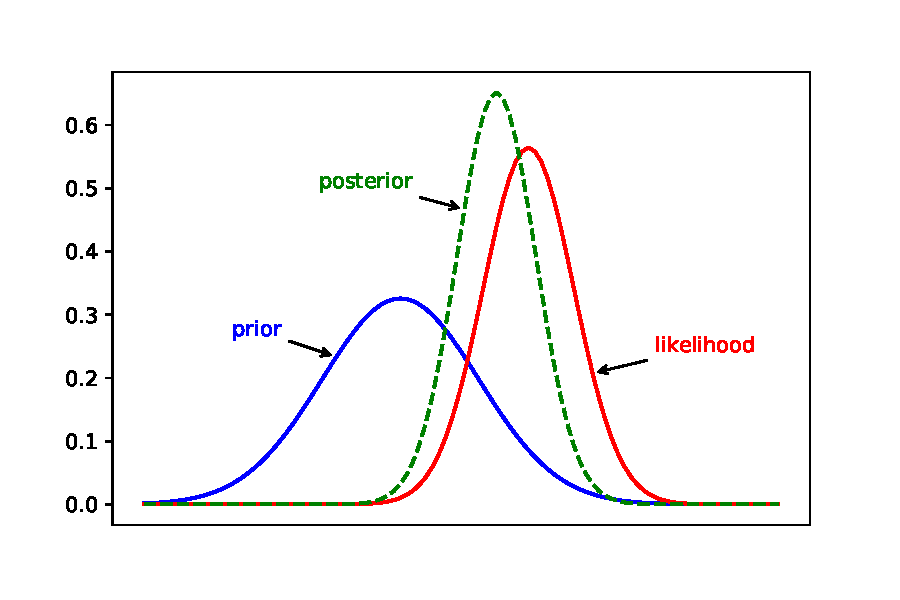
\includegraphics[width=0.45\textwidth]{Imagens/gauss_fusion.pdf}}
	\subfigure[]{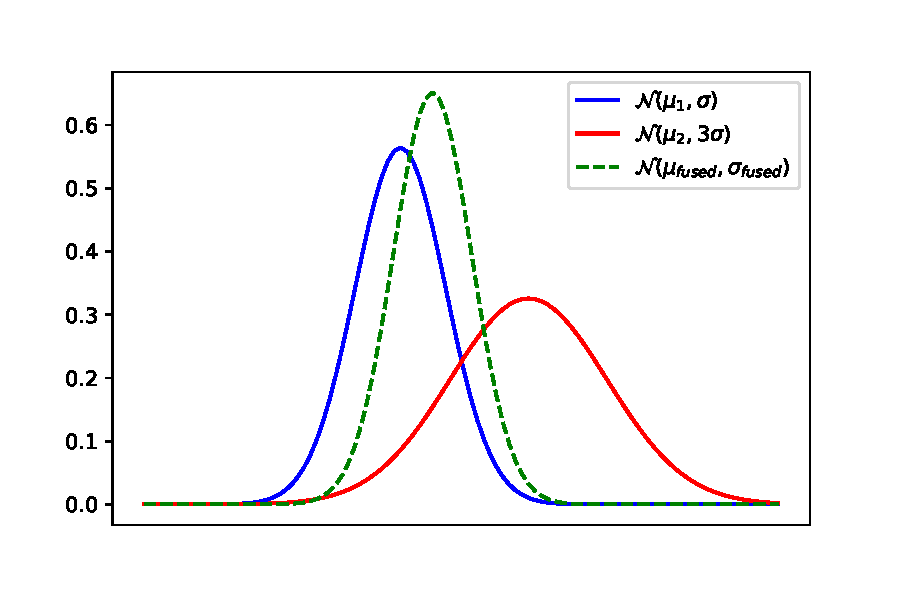
\includegraphics[width=0.45\textwidth]{Imagens/gauss_fusion2.pdf}}
	\caption[\textit{Posterior} density obtained by the fusion \textit{prior} and \textit{likelihood}]{\textit{Posterior} density obtained by the fusion of \textit{prior} and \textit{likelihood} densities. In (a) the variance of the \textit{likelihood} is smaller than the variance of the \textit{prior}, hence the \textit{posterior} is closer to the \textit{likelihood}. In (b) is the other way around.}
	\label{fig:gauss_fusion}
\end{figure}

\subsection{Kalman Filter}\label{sec:kalman-filter}

The Bayesian recursive solution described by proposition~\ref{prop:bayes_solution} enables the computation of the optimal estimation of state vector $x_k$. However, its implementation is impossible for practical applications, since it relies on mathematical integrations and as time evolves, the observation sequence grows indefinitely. The sequential algorithm proposed by \citep{Kalman1960} solves that problem adding a restriction in the system assumptions, that is linearity and Gaussianity. 

Consider the Gauss-Markov discrete-time linear system

\begin{align}
x_k &= A_{k-1}x_{k-1} + B_{k-1}u_{k-1} + G_{k-1}w_{k-1}, \label{eq:gm_process}\\
y_k &= C_kx_k+ v_k, \label{eq:gm_obs}
\end{align}

\noindent
where, $\forall k \geq1$, time varying matrices $A_{k-1} \in \mathbb{R}^{n\times n}$,  $B_{k-1} \in \mathbb{R}^{n\times p}$,  $G_{k-1} \in \mathbb{R}^{n\times q}$ and  $C_{k-1} \in \mathbb{R}^{m\times n}$ are known, as well as the input $u_{k-1} \in \mathbb{R}^P$ and output $y_k \in \mathbb{R}^m$ vectors. Process and observation noise vectors, $w_{k-1} \in \mathbb{R}^q$ and $v_{k-1} \in \mathbb{R}^m$ are white, zero-mean and mutually independent, apart from being Gaussian, with known covariance matrices $Q_{k-1}$ and $R_k$, respectively.

Define $\mathcal{N}(x;\mu,\Sigma)$ as a multivariate Gaussian probability density function on $x$, with mean $\mu$ and covariance $\Sigma$, given by

\begin{equation}
\mathcal{N}(x;\mu,\Sigma) = \frac{1}{(2\pi)^{n/2} \left| \Sigma \right|^{1/2}}exp\left( -\frac{1}{2}(x-\mu)^T \Sigma^{-1}(x-\mu)\right)
\end{equation}

Some identities of multivariate Gaussian probability densities are needed for the next steps and are described in properties ~\ref{prop:joint} and~\ref{prop:marginal}.

\begin{prop} \label{prop:joint}
	If the random variables $x$ and $y$ have the joint Gaussian probability density
	
	\begin{align}
	x,y \sim \mathcal{N} 
	\left(
	\begin{pmatrix} x \\ y \end{pmatrix};
	\begin{pmatrix} a \\ b \end{pmatrix},
	\begin{pmatrix} A & C\\ C^T & B \end{pmatrix}
	\right) 
	\end{align}
	
	\noindent
	then, the marginal and conditional densities of $x$ and $y$ are given by
	
	\begin{align}
	x 		&\sim \mathcal{N}(x;\ a,A) \\
	y 		&\sim \mathcal{N}(y;\ b,B) \\
	x|y  	&\sim \mathcal{N}(x; \ a + CB^{-1}(y-b),\ A - C B^{-1} C^T ) \\
	y|x  	&\sim \mathcal{N}(y; \ b + C^T A^{-1}(x-a),\  B - C^T A^{-1} C)
	\end{align}
	
\end{prop}

\begin{prop} \label{prop:marginal}
	
	If the random variables $x$ and $y$ have the Gaussian densities
	\begin{align}
	\rho(x) 	&= \mathcal{N}(x;\ a, \ A), \\
	\rho(y|x) 	&= \mathcal{N}(y;\ Hx, \ B),
	\end{align}
	
	Then, the joint and marginal densities are given by
	
	\begin{align}
	x,y &\sim \mathcal{N} 
	\left(
	\begin{pmatrix} x \\ y \end{pmatrix};
	\begin{pmatrix} a \\ Ha \end{pmatrix},
	\begin{pmatrix} A & AH^T\\ HA & HAH^T + B \end{pmatrix}
	\right), \\
	y &\sim \mathcal{N} (y; \ Ha, \ HAH^T + B)
	\end{align}
\end{prop}


From the Gauss-Markov assumptions, we can rewrite (\ref{eq:gm_process}) and (\ref{eq:gm_obs}) from a probabilistic perspective, as

\begin{align}
\rho(x_k|x_{k-1}) &= \mathcal{N}(x_k ; \ A_{k-1}x_{k-1} + B_{k-1}u_{k-1}, \ Q_k), \label{eq:rho_process}\\
\rho(y_k|x_k) &= \mathcal{N}(y_k; \ C_kx_k, \ R_k), \label{eq:rho_obs}
\end{align}

\noindent
where (\ref{eq:rho_process}) is the \textit{transition} density representing the system dynamics and (\ref{eq:rho_obs}) is the \textit{likelihood} density, given by the observation model. 

The Bayesian recursive solution to such system is defined by \textit{forecast} and \textit{data assimilation} steps according to

\begin{align}
\rho(x_{k}|(y_1,...,y_{k-1}) &= \mathcal{N}(x_k; \ \hat{x}_{k|k-1},P^{xx}_{k|k-1}), \label{eq:sol_xk}\\
\rho(x_{k}|(y_1,...,y_{k}) &= \mathcal{N}(x_k; \ \hat{x}_{k|k},P^{xx}_{k|k}) \label{eq:sol_xk1},
\end{align}

\noindent
with the \textit{posterior} density function from a previous step given by

\begin{equation}
\rho(x_{k-1}|(y_1,...,y_{k-1}) = \mathcal{N}(x_{k-1}; \ \hat{x}_{k-1|k-1},P^{xx}_{k-1|k-1}), \label{eq:previous}
\end{equation}

\noindent
where $\hat{x}_{k|k-1}$ and $P^{xx}_{k|k-1}$ are the \textit{forecast} state and covariance estimates, whereas $\hat{x}_{k|k}$ and $P^{xx}_{k|k}$ are the \textit{data assimilation} state and covariance estimates.

Now we combine the \textit{forecast steps} from (\ref{eq:prop_xk1}) and from (\ref{eq:sol_xk}), using the process model from (\ref{eq:rho_process}), the previous estimate from (\ref{eq:previous}) and the identities from property~\ref{prop:marginal}, yielding

\begin{align}
\rho(x_k|(y_1,...,y_{k-1})) &= \int_{\mathbb{R}^n}\rho(x_k|x_{k-1}) \rho(x_{k-1}|y_1,...,y_{k-1})dx_{k-1}, \label{eq:forecast}\\
							&= \mathcal{N}(x_k; \ A_{k-1}\hat{x}_{k-1|k-1} + B_{k-1}u_{k-1}, \ A_{k-1}P^{xx}_{k-1|k-1}A{k-1}^T + G_{k-1}QG_{k-1}^T, \notag
\end{align}

\noindent
that is, the \textit{forecast} state and covariance estimates are computed by

\begin{align}
\hat{x}_{k|k-1} &= A_{k-1}\hat{x}_{k-1|k-1} + B_{k-1}u_{k-1}, \label{eq:forecast_state} \\
P^{xx}_{k|k-1}	&= A_{k-1}P^{xx}_{k-1|k-1}A{k-1}^T + G_{k-1}QG_{k-1}^T. \label{eq:forecast_cov}
\end{align}

And for the \textit{data assimilation step}, we find the joint density of $y_k$ with the \textit{forecast} estimate from (\ref{eq:forecast}), using property~\ref{prop:joint}

\begin{equation}
\rho(x_k,y_k|(y_1,...,y_{k-1})) = \mathcal{N} 
\left(
\begin{pmatrix} x_k \\ y_k \end{pmatrix}; \
\begin{pmatrix} \hat{x}_{k|k-1} \\ C_k\hat{x}_{k|k-1} \end{pmatrix},
\begin{pmatrix} P^{xx}_{k|k-1} & P^{xx}_{k|k-1}C_k^T\\ C_kP^{xx}_{k|k-1} & C_k P^{xx}_{k|k-1} C_k^T + R_k \end{pmatrix}
\right),	
\end{equation}

\noindent
and the marginal density for $x_k$ is

\begin{equation}
\rho(x_{k}|(y_1,...,y_{k})) = \mathcal{N}(x_k; \ \hat{x}_{k|k-1}+K_k(y_k-C_k\hat{x}_{k|k-1}),P^{xx}_{k|k-1}-P^{xx}_{k|k-1}C_k^T K_k^{-1}P^{xx}_{k|k-1}C_k^T),
\end{equation}
\noindent
that is, the \textit{data assimilation} state and covariance estimates are calculated by

\begin{align}
\hat{x}_{k|k} &= \hat{x}_{k|k-1}+K_k(y_k-C_k\hat{x}_{k|k-1}), \label{eq:assim_state}\\
P^{xx}_{k|k}	&= P^{xx}_{k|k-1}-P^{xx}_{k|k-1}C_k^T K_k^{-1}P^{xx}_{k|k-1}C_k^T. \label{eq:assim_cov}
\end{align}

\noindent
where $K_k \in \mathbb{R}^{n\times m}$ is defined as the Kalman gain and is given by

\begin{equation} \label{eq:kalman_gain}
K_k = P^{xx}_{k|k-1}C_k^T(C_kP^{xx}_{k|k-1}C_k^T + R_k)^{-1}.
\end{equation}

If we define a \textit{forecast} output estimate $\hat{y}_{k|k-1}$, an innovation covariance matrix $P^{yy}_{k|k-1}$ and a cross-covariance matrix $P^{xy}_{k|k-1}$ as 

\begin{align}
\hat{y}_{k|k-1} &\triangleq C_k\hat{x}_{k|k-1}, \\
P^{yy}_{k|k-1} 	&\triangleq E\left[ (y_k-\hat{y}_{k|k-1})(y_k-\hat{y}_{k|k-1})^T \right] = C_kP^{xx}_{k|k-1}C_k^T + R_k , \\
P^{xy}_{k|k-1}	&\triangleq E\left[ (x_k  - \hat{x}_{k|k-1})(y_k-\hat{y}_{k|k-1})^T\right] = P^{xx}_{k|k-1}C_k^T , \\
\end{align}

\noindent
we can simplify \textit{data assimilation} step given by (\ref{eq:assim_state}), (\ref{eq:assim_cov}) and (\ref{eq:kalman_gain}) as

\begin{align}
\hat{x}_{k|k} 	&= \hat{x}_{k|k-1}+K_k(y_k-\hat{y}_{k|k-1}), \label{eq:assim_state2} \\
P^{xx}_{k|k}	&= P^{xx}_{k|k-1}-P^{yy}_{k|k-1} K_k^{-1} (P^{yy}_{k|k-1})^T, \label{eq:assim_cov2} \\
K_k 			&= P^{xy}_{k|k-1}(P^{yy}_{k|k-1})^{-1}. \label{eq:kalman_gain2}
\end{align}


For more details on this derivation, refer to \citep{Sarkka2013}. We summarize the Kalman filter algorithm as below
\begin{algo} \label{alg:KF}Kalman filter (KF) algorithm.
\begin{quote}
\textit{Forecast step}: Using the linear model, calculate the estimated state vector $\hat{x}_{k|k-1}$ and the estimated state covariance $P^{xx}_{k|k-1}$, using (\ref{eq:forecast_state}) and (\ref{eq:forecast_cov}). Calculate Kalman gain $K_k$ by (\ref{eq:kalman_gain}).
\end{quote}
\begin{quote}
\textit{Data assimilation step}: Using the measurement vector $y_k$ and Kalman gain, update estimations from previous step with (\ref{eq:assim_state}) and (\ref{eq:assim_cov}), obtaining estimates $\hat{x}_{k|k}$ and $P^{xx}_{k|k}$.
\end{quote}
\end{algo}

The linear KF is the optimal estimator under both MAP and MMSE criteria, it is unbiased and its cross-covariance will asymptotically achieve the lower bound of the Cram�r-Rao inequality \citep{Teixeira2008}.


\subsection{Unscented Kalman Filter}\label{sec:unscented-kalman-filter}	

For non-linear systems, the Gaussianity requirement does not hold, even if the uncertainty and initial conditions are Gaussian. Therefore, we can not characterize the posterior PDF only by its first two moments, mean and covariance, and the solution given by proposition~\ref{prop:bayes_solution} are not suited for the estimation problem. In fact, optimal solutions are generally not possible to be obtained by a recursive algorithm.

Adaptations to the Kalman filter have been proposed in the literature. The extended Kalman filter (EKF), for example, linearizes the system around the state estimates, to achieve approximations through algorithm~\ref{alg:KF}. A different approach is to approximate the statistics of the posterior PDF, instead of the model. The unscented Kalman filter (UKF) \citep{Julier2004} performs statistical approximations via the unscented transformation (UT), addressing many of the drawbacks that appear in the EKF implementation, such as the necessity of differentiability, the performance loss due to systems that are poorly approximated by linearization and computational efficiency. Therefore the UKF is the chosen method for the non-linear system state estimation simulated in Chapter~\ref{cap5} and will be further discussed in this section.

Based on the Monte Carlo approach to statistical approximation, we define a set of samples $\chi \triangleq [\chi_0,...,\chi_{2n+1}] \in \mathbb{R}^{n\times (2n+1)}$, also referred to as sigma points, to approximate the mean $\bar{x}$ and covariance $\bar{P}^{xx}$ of the random variable being estimated, such that

\begin{align}
\sum_{j=0}^{2n+1} \gamma_j\chi_j &= \bar{x}, \\
\sum_{j=0}^{2n+1} \gamma_j\left[ (\chi_j-\bar{x})(\chi_j-\bar{x})^T \right] &= \bar{P}^{xx}, \\
\sum_{j=0}^{2n+1} \gamma_j &= 1.
\end{align}

\noindent
where $\gamma_{j}$, $\forall j > 1$ are called weights. Then, the original UT proposed by \citep{Julier1997} determines the choice of sigma points by

\begin{align}
\chi_0 		&= \bar{x}, \\
\chi_i 		&= \bar{x} + \left(\sqrt{(n+\kappa)\bar{P}^{xx}} \right)_i \ , \\
\chi_{i+n} 	&= \bar{x} - \left(\sqrt{(n+\kappa)\bar{P}^{xx}} \right)_i \ ,
\end{align}

\noindent
and weights by

\begin{align}
\gamma_0 		&= \frac{\kappa}{n+\kappa} \  , \\
\gamma_i 		&= \frac{1}{2(n+\kappa)} \ , \\
\gamma_{i+n} 	&= \frac{1}{2(n+\kappa)} \ .
\end{align}

\noindent
where $n$ is the dimension of the random state vector and the scaling factor $\kappa$ provides a tunning degree of freedom to approximate higher order moments of the random variable given by the state vector $x_k$.

For this study we will adopt a simplified version of the UKF, with $\kappa = 0$. In other words, sigma points are defined as

\begin{align}
\chi \triangleq \left[\bar{x} 1_{1\times(2n+1)}+\sqrt{n} (\bar{P}^{xx})^{1/2} \quad \bar{x} 1_{1\times(2n+1)}-\sqrt{n}(\bar{P}^{xx})^{1/2}\right],
\end{align}

\noindent
with weights given by

\begin{align}
\gamma = \frac{1}{2n},
\end{align}

Based on this approximations, and considering the process and observation models given by (\ref{eq:prob_process}) and (\ref{eq:prob_obs}), the UKF algorithm is defined by

\begin{algo} \label{alg:UKF} Unscented Kalman filter (UKF) algorithm.
	
\noindent
\textit{Forecast step}: Calculate sigma points $\chi_{j,k|k-1}$ based on last estimation and use them to forecast state estimate $\hat{x}_{k|k-1}$ and the respective covariance $P^{xx}_{k|k-1}$ via the UT.
\begin{align}
\chi_{k-1|k-1} 	&= \left[\hat{x}_{k-1|k-1}1_{1\times(2n+1)}+\sqrt{n} (P^{xx}_{k-1|k-1})^{1/2} \quad\hat{x}_{k-1|k-1}1_{1\times(2n+1)} -\sqrt{n}(P^{xx}_{k-1|k-1})^{1/2}\right], \\
\chi_{j,k|k-1} 	&= f(\chi_{j,k-1|k-1},u_{k-1},k-1), \quad j=1,...,2n+1, \\
\hat{x}_{k|k-1}	&= \sum_{j=1}^{2n+1}\gamma\chi_{j,k|k-1}, \\
P^{xx}_{k|k-1}	&= \sum_{j=1}^{2n+1}\gamma \left[ (\chi_{j,k|k-1}-\hat{x}_{k|k-1})(\chi_{j,k|k-1}-\hat{x}_{k|k-1})^T\right]+ G_{k-1}QG_{k-1}^T.
\end{align}
Calculate new forecast state sigma points $\chi_{k|k-1}$ based on forecast state estimate $\hat{x}_{k|k-1}$ and find forecast observation sigma points $\Upsilon_{j,k|k-1}$. Propagate them to an estimated observation vector $\hat{y}_{k|k-1}$, using the observation model. Calculate observation vectors covariance $P^{yy}_{k|k-1}$ and the cross-covariance between observation and state $P^{xy}_{k|k-1}$.
 
\begin{align}
\chi_{k|k-1} 	&= \left[\hat{x}_{k|k-1}1_{1\times(2n+1)}+\sqrt{n} (P^{xx}_{k|k-1})^{1/2} \quad\hat{x}_{k|k-1}1_{1\times(2n+1)} -\sqrt{n}(P^{xx}_{k|k-1})^{1/2}\right], \\
\Upsilon_{j,k|k-1} 	&= g(\chi_{j,k|k-1},k), \quad j=1,...,2n+1, \\
\hat{y}_{k|k-1}	&= \sum_{j=1}^{2n+1}\gamma\Upsilon_{j,k|k-1}, \\
P^{yy}_{k|k-1}	&= \sum_{j=1}^{2n+1}\gamma \left[ (\Upsilon_{j,k|k-1}-\hat{y}_{k|k-1})(\Upsilon_{j,k|k-1}-\hat{y}_{k|k-1})^T\right]+ R_k. \\
P^{xy}_{k|k-1}	&= \sum_{j=1}^{2n+1}\gamma \left[ (\chi_{j,k|k-1}-\hat{x}_{k|k-1})(\Upsilon_{j,k|k-1}-\hat{y}_{k|k-1})^T\right].
\end{align}


\noindent
\textit{Data assimilation step}: Calculate Kalman gain and finish the estimation of state estimate and covariance at time $k$.
	
 
\begin{align}
K_k					&= P^{xy}_{k|k-1} (P^{yy}_{k|k-1})^{-1}, \\
\hat{x}_{k|k} 	&= \hat{x}_{k|k-1} + K_k(y_k - \hat{y}_{k|k-1}),	 \\
P^{xx}_{k|k}		&= P^{xx}_{k|k-1} - P^{yy}_{k|k-1} K_k^{-1} (P^{yy}_{k|k-1})^T.
\end{align}

\end{algo}



	
\section{State Estimation with Aperiodic Sampling} \label{sec:estimation_aperiodic}

In general, state estimation in sampled-data systems are designed considering regular sampling time intervals. However, we are interested in the effects of aperiodic sampling and data assimilation executed at incorrect time instants, as formulated in Section~\ref{sec:problem_form}. 

First, we note that the measurement instants $t_k$, $\forall k \in \mathbb{N}$ do not match the estimation instants $iT$, $\forall i \in \mathbb{N}$. Additionally, input data $u(iT)$ is available a rate $1/T$ that is $\alpha > 1$ times faster than the expected sampling rate $\lambda_h$ of the observations. Therefore, there are time intervals $iT - (i-1)T$ without any observations, hence only the \textit{forecast} step of state estimation can be performed. One example of such application is in target tracking, where inertial sensors that measure process input data such as linear acceleration and angular velocity operate at higher frequencies compared to GPS sensors, that are responsible for the observation model data.

An illustrative example is presented in Figure~\ref{fig:cap4-sampling_example}, where $\alpha=5$, that is the expected time interval for observations $1/\lambda_h$ is five times higher than regular sampling time interval $T$. Between two consecutive estimation time instants, there can be no observation data, illustrated by the red letter \textit{A}, there can be one measurement, red letter \textit{B}, or multiple measurements, shown in the red letter \textit{C}.


\begin{figure}[!htb]
	\centering
	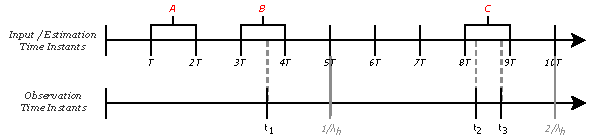
\includegraphics[width=\textwidth]{Imagens/cap4-sampling_example.pdf}
	\caption[Input and observation time instants realization]{Input and estimation time instants labeled as $iT$ and a realization of observation time instants, labeled as $t_k$. Expected time instants for observation is presented in gray, considering that $E[d_k] = \frac{1}{\lambda_h}$, and $\frac{1}{\lambda_h} = 5 T$, that is $\alpha=5$.}
	\label{fig:cap4-sampling_example}
\end{figure} 

On the next subsections, we discuss how the algorithm is executed for the scenarios when reliable time-stamp information is available, and when it is not present in the information package.

%\subsection{Input Irregular Sampling}
%
%Em caso de amostragem irregular tamb�m na entrada, um esquem�tico dos instantes de estima��o, amostragem e entrada pode ser observado na Fig.~\ref{fig:esquema2}
%
%\begin{figure}[!htb]
%	\centering
%	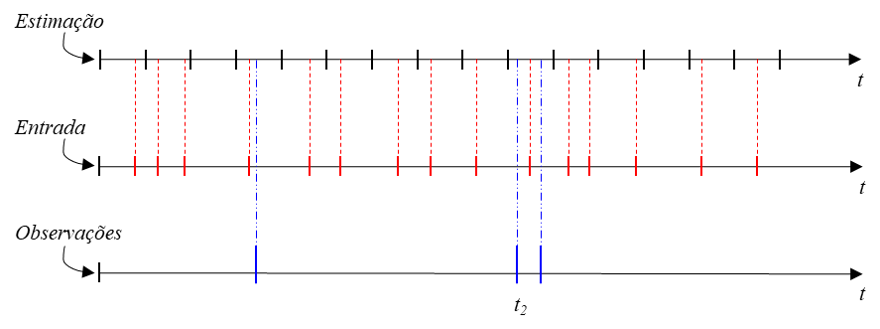
\includegraphics[scale=0.65]{Imagens/esquema3}
%	\caption[Exemplos de instantes de amostragem de estima��o]{Exemplos de instantes de amostragem de estima��o(1), da entrada (2) e das observa��es (3). Os instantes m�ltiplos de $\lambda$, igual ao intervalo m�dio de amostragem das observa��es s�o apresentados em cinza escuro, para refer�ncia.}
%	\label{fig:esquema2}
%\end{figure} 
%
%Para atrasos de transmiss�o:
%
%\begin{figure}[!htb]
%	\centering
%	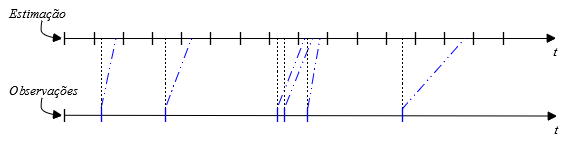
\includegraphics[scale=0.65]{Imagens/esquema4}
%	\caption[Exemplos de instantes de amostragem de estima��o com atraso de tempo]{Exemplos de instantes de amostragem de estima��o(1), da entrada (2) e das observa��es (3). Os instantes m�ltiplos de $\lambda$, igual ao intervalo m�dio de amostragem das observa��es s�o apresentados em cinza escuro, para refer�ncia.}
%	\label{fig:esquema3}
%\end{figure} 
%
%Nas pr�ximas subse��es � apresentado como os algoritmos de estima��o tratam os cen�rios \textbf{A}, \textbf{B} e \textbf{C} para os casos em que o carimbo de tempo est� e n�o est� dispon�vel.
%

\subsection{With Timestamp}\label{sec:carimbo}

If the estimator knows the exact time $t_k$ that measurements were taken in a global timescale, \textit{data assimilation} steps can be performed at the correct time instants. For that, the process model defined by (\ref{eq:prob_process}) needs to discretized at variable time intervals $\delta t_j^*$, yielding

\begin{equation}\label{eq:disc_carimbo}
x(t^*_j)=f_\textrm{d}(x(t^*_{j-1}),u(t^*_{j-1}),w(t^*_{j-1}),t^*_{j-1}),
\end{equation}

\noindent
where $t^*_j= t^*_{j-1} + \delta t^*_j$ and $t^*_0=0$. Each value $\delta t^*_j$ corresponds to the time interval between the last instant $t^*_{j-1}$ in which a signal was received, whether it transmitted input or observation data, and the next time interval $t^*_{j}$ in which a new signal arrives. A zero order holder (ZOH) is used between observation and input signals, considering last available information. Note that in such configuration, the discrete-time system becomes time-varying, since discretization is performed using variable time intervals. For the simulation carried out in Section~\ref{cap5}, time intervals $\delta t^*_j$ are calculated by uniting all arrival times for input and observation in a single vector, in an orderly fashion. The subtraction of consecutive time instants yields the time intervals sequence $\delta t^*_j$, $\forall j \geq 1$. 

Since there are two signal types, input and observation, there are four possible cases for the estimator: input followed by another input; input followed by an observation; observation followed by an input; and observation followed by another observation. In Figure~\ref{fig:cap4-sampling_example}, all of them are represented. During the interval \textit{A}, there are only input signals, so time interval is $T$ and only \textit{forecast} is performed. In the interval represented by \textit{B}, we have to first execute complete \textit{forecast} and \textit{data assimilation} steps between input and observation, from $3T$ until $t_1$, using $\delta t^*_4 =t_1-3T$. Next, between an observation and an input signal, a ZOH is used for a \textit{forecast} step between $t_1$ and $4T$. In other words, it is considered that the input remained constant between $3T$ and $4T$. When more than one observation arrive between two input signals, as in \textit{C}, full \textit{forecast} and \textit{data assimilation} are performed as many times needed before one last \textit{forecast} between the last observation and the next input signal.

For the \textit{online} estimator, the differential equations are numerically integrated as input or measurement signals arrive. In these instants, the corresponding time interval $\delta t^*_j$ is calculated. If the current signal transmits input data, only the \textit{forecast} step is executed. If it is observation data being received, both \textit{forecast} and \textit{data assimilation} steps are performed, considering a ZOH for the input data. This process is illustrated in Figure~\ref{fig:cap4-online_estimator}.

\begin{figure}[!htb]
	\centering
	\begin{adjustbox}{width=0.65\textwidth,height=\textheight,keepaspectratio}
		
		\begin{tikzpicture}[node distance=2cm, font = \scriptsize]
		
		\node(start)[startstop][text width=2.8cm,align=center]{\textbf{Start} \\ $t^*_0=0$; \\ $i=j=k=1$; \\};
		
		\node (dec1) [decision, below of=start,yshift=-0.5cm] {Signal Received};
		
		\node (pro1) [process, below right of=dec1, yshift=-0.9cm, xshift=0.25cm][text width=2.8cm,align=center]{Calculate \\ $\delta t^*_{j} = iT - t^*_{j-1}$ \\ $t^*_{j} = t^*_{j-1} + \delta t^*_{j}$};
		
		\node (pro12) [process, below of=pro1][text width=2.8cm,align=center, yshift=0.5cm]{Forecast Step};
		
		\node (pro2) [process, below left of=dec1,  yshift=-0.9cm, xshift=-0.25cm][text width=2.8cm,align=center]{Calculate \\ $\delta t^*_{j} = t_k - t^*_{j-1}$ \\ $t^*_{j} = t^*_{j-1} + \delta t^*_{j}$};
		
		\node (pro22) [process, below of=pro2][text width=2.8cm,align=center, yshift=0.5cm]{Forecast Step, using ZOH};
		
		\node (pro23) [process, below of=pro22][text width=2.8cm,align=center, yshift=0.7cm]{Data Assimilation \\ Step};
		
		\node (pro3) [startstop, below of = pro23][text width=2.8cm,align=center, xshift=1.8cm]{Estimate in $t^*_{j}$};
		
		\draw [arrow] (start) -- node[pos=0.5](h){} (dec1);
		\draw [arrow] (dec1) -| node[text width=2.8cm,align=center,anchor=west,xshift=-1cm] {Iput \\ Signal} (pro1);
		\draw [arrow] (dec1) -| node[text width=2.8cm,align=center,anchor=east,xshift=0.8cm] {Observation\\ Signal} (pro2);
		\draw [arrow] (pro1) -- (pro12);
		\draw [arrow] (pro2) -- (pro22);
		\draw [arrow] (pro22) -- (pro23);
		\draw [arrow] (pro12) -- node[text width=2.8cm,align=center,anchor=south,xshift=0.8cm, yshift=-1cm] {$i=i+1$} (pro3);
		\draw [arrow] (pro23) -- node[text width=2.8cm,align=center,anchor=east,xshift=0.6cm] {$k=k+1$}(pro3);
		\draw [arrow] (pro3) --+(-4cm,0) |- node[text width=2.8cm,align=center,anchor=south,xshift=1cm] {$j=j+1$}(h);
		\end{tikzpicture}
	\end{adjustbox}
	
	\caption[Illustrative schematic of the \textit{online} estimator, with time-stamp]{Illustrative schematic of the \textit{online} estimator, with time-stamp. Indexes $i$, $j$ e $k$ represent the input, estimation and observation signal counters, respectively.}
	\label{fig:cap4-online_estimator}
\end{figure}	

\subsection{Without Timestamp}

On the other hand, in case there is no information about time-stamp, process model (\ref{eq:prob_process}) is discretized according to


\begin{equation}\label{eq:disc_semcarimbo}
x_n=f^*_\textrm{d}(x_{n-1},u_{n-1},w_{n-1},n),
\end{equation}

\noindent
where $t=nT$.

Since the estimator is not aware of the measurement time instant, \textit{data assimilation} is always performed as the next input signal arrives, in a time instant multiple of $T$. In such cases, there are only two possible scenarios. One, in which there are no information between two consecutive input signal arrivals, represented by the letter \textit{A} in Figure~\ref{fig:cap4-sampling_example}, when only \textit{forecast} step is performed. If there is observation, full \textit{forecast} and \textit{data assimilation} steps are performed, considering the time interval $T$. In case illustrated by the letter \textit{B}, measurement taken at time $t_1$ will be assimilated in time instant $4T$. When there are multiple measurements between two input signals, the oldest ones are discarded, as in letter \textit{C}, for which the measurement taken at $t_2$ is discarded and the one taken at $t_3$ is assimilated at the instant $9T$.

\clearpage
\section{State Estimation Performance Metrics} \label{sec:metrics}

In order to assess the performance degradation introduced by assimilating data at incorrect time instants, we need to define certain performance metrics for comparison. The algorithms described in Sections~\ref{sec:unscented-kalman-filter} and~\ref{sec:kalman-filter} estimate both the current state, $\hat{x}_{k|k}$ and its covariance matrix $\hat{P}^{xx}_{k|k}$. For the linear case, the \textit{posterior} conditional PDF 
$\rho(x_{k}|(y_1,...,y_{k})$ is Gaussian, according to (\ref{eq:sol_xk1}), so it is fully characterized by its two first moments. Thus, if the filter is consistent, the following conditions shall be met \citep{Bar-Shalom2001}

\begin{align}
E\left[x_k - \hat{x}_{k|k}\right] &\triangleq E[\tilde{x}_{k|k}] = 0, \label{eq:consistency1} \\
E\left[(x_k - \hat{x}_{k|k})(x_k - \hat{x}_{k|k})^T\right] &\triangleq E[\tilde{x}_{k|k}\tilde{x}_{k|k}^t] = P^{xx}_{k|k}, \label{eq:consistency2}
\end{align}

\noindent
where $\tilde{x}_{k|k}$ is the estimation error at time instant $k$. Condition (\ref{eq:consistency1}) is called \textit{unbiasedness} requirement, whereas (\ref{eq:consistency1}) refers to \textit{covariance matching}. For the non-linear case, these conditions cannot be fully met, since the \textit{posterior} PDF is an approximation of a Gaussian density. Thus, the closer they are met, the more consistent are the filter results.

In this study we will use metrics that measure both consistency conditions. According to Bar-Shalom, in order to test them, the consistency criteria metrics for state estimation must certify: that state estimate errors are zero mean and compatible with the estimated state covariance; that innovations are also zero mean and compatible with their respective covariances; and that innovations are white. We will adopt two tests proposed by him that attests all conditions simultaneously, that is the normalized (state) estimation error squared (NEES) and normalized innovation squared (NIS) tests. We first defined NEES and NIS as


\begin{align}
NEES_k &\triangleq  \tilde{x}_{k|k}^T(P^{xx}_{k|k})^{-1}\tilde{x}_{k|k}, \label{eq:nees} \\
NIS_k &\triangleq  \eta_{k|k-1}^T(P^{yy}_{k|k-1})^{-1}\eta_{k|k-1}, \label{eq:nis}.
\end{align}

Under the linear and Gaussian assumption, we formulate a hypothesis test, under which the null hypothesis $H_0$, that the filter is consistent, requires that both NEES and NIS follow chi-squared distributions, with $n_x$ and $n_y$ degrees of freedom, respectively, and $n_x$ is the dimension of the state vector, whereas $n_y$ is the dimension of the observation vector. The expected value of a RV that is chi-squared distributed is equal to its degrees of freedom quantity, that is $E[NEES_k] = n_x, \ \forall k > 1$ and  $E[NIS_k] = n_y, \ \forall k > 1$. 

We adopt single-run tests, thus for every estimation, we test the acceptance of $H_0$, that is if both NEES and NIS at time instants $k$ are within a certain interval, considering the accepted region as 

\begin{align}
P \left\{ NEES_k \in [r_1,r_2] | H_0 \right\} &= 1 - \alpha, \label{eq:nees_h0} \\
P \left\{ NIS_k \in [r_1,r_2] | H_0 \right\} &= 1 - \alpha, \label{eq:nis_h0}
\end{align}

\noindent
where $\alpha$ is the significance level and interval $[r_1,r_2]$ is given by the chi-square distribution degrees of freedom and $\alpha$. For instance, considering a system with a state vector of size 4 and observation vector of size 1, and a significance level of $\alpha=5\%$, the acceptance intervals for NEES and NIS are respectively given by

\begin{align}
\left[\chi^2_1(0.025),\ \chi^2_1(0.975)\right] &= [0.001, \ 5.02], \label{eq:nees_interval} \\
\left[\chi^2_4(0.025),\ \chi^2_4(0.975)\right] &= [0.484, \ 11.1], \label{eq:nis_interval}
\end{align}

\noindent
which means that, if the filter is consistent, in $95\%$ of the estimates, NEES and NIS value should fall under their correspondent intervals.

Additionally, since we are using simulated systems, the root mean square error (RMSE) of the system states will also be calculated as an accuracy performance index, given by


\begin{equation}\label{eq:rmse}
RMSE = \frac{ \sum_{i=1}^N \sqrt{(\hat{x}_{k|k}-x_{k})^2}}{N}
\end{equation}

\noindent
where $x_k$ is the true state vector and $N$ is the amount of estimates.

\clearpage